% !TeX spellcheck = es_ANY
% Chapter 1

%\chapter{Chapter Title Here} % Main chapter title
%
%\label{Chapter1} % For referencing the chapter elsewhere, use \ref{Chapter1} 

%----------------------------------------------------------------------------------------

% Define some commands to keep the formatting separated from the content 
%\newcommand{\keyword}[1]{\textit{#1}}
%\newcommand{\tabhead}[1]{\textbf{#1}}
%\newcommand{\code}[1]{\texttt{#1}}
%\newcommand{\file}[1]{\texttt{\bfseries#1}}
%\newcommand{\option}[1]{\texttt{\itshape#1}}

%----------------------------------------------------------------------------------------

\chapter{Calibraci\'on Qu\'imica}
	La calibraci\'on qu\'imica consiste en contrastar las propiedades termodin\'amicas de un sistema qu\'imico, obtenidas usando el calor\'imetro con aquellas reportadas en la literatura. Para esto se estudia la reacci\'on del \'acido clorhidrico con bicarbonato de potasio. Esta reacci\'on presenta varias ventajas: por un lado hace uso de reactivos de f\'acil acceso, es una reacci\'on con esqueometr\'ia 1:1, ha sido estudiada previamente, y adem\'as, es usada en calibraciones de equipos calorim\'etricos., como el calor\'imetro de titulaci\'on NanoITC de \textit{TA instruments}.
	
\section{Preparaci\'on de las soluciones de HCl}
	Para la preparaci\'on de las soluciones, se hace uso de forma sistem\'atica de una balanza XXXX y un dens\'imetro YYYY. Adem\'as, en el proceso de preparaci\'on se hace necesaria la toma de dos al\'icuotas de 30 $\mu$L y 170 $\mu$L, para el HCl y \ce{KHCO3} correspondientemente, por lo cual se usa una micropipeta ZZZZ con rango de 20 a 200 $\mu$L.
	\subsection{Soluci\'on de HCl 0.25 mM}
		Para determinar la concentraci\'on de una soluci\'on de 1.0 mL de HCl concentrado en 25.0 mL de agua tipo 1, se midi\'o la densidad de la soluci\'on, posteriormente usando como referencia los datos reportados en la literatura fue realizada una regresi\'on lineal que permiti\'o relacionar la concentraci\'on con la densidad de la soluci\'on $\rho$ \cite{perry2007perry}. De esta manera se estableci\'o el valor de la concentraci\'on en: $3.02 \pm 0.05$ \% (fracci\'on de masa $[w_t]$), donde la incertidumbre se obtiene de la pendiente ($m$) e intercepto ($b$) de la regresi\'on lineal que se muestra en la \autoref{fig: HCl_density}.
		\begin{equation}
			\delta [w_t] = \sqrt{\left(\dfrac{\rho-b}{m^2}\delta m\right)^2 + \left(\dfrac{\delta b}{m}\right)^2}
		\end{equation}
		\begin{figure}[h]
			\centering
			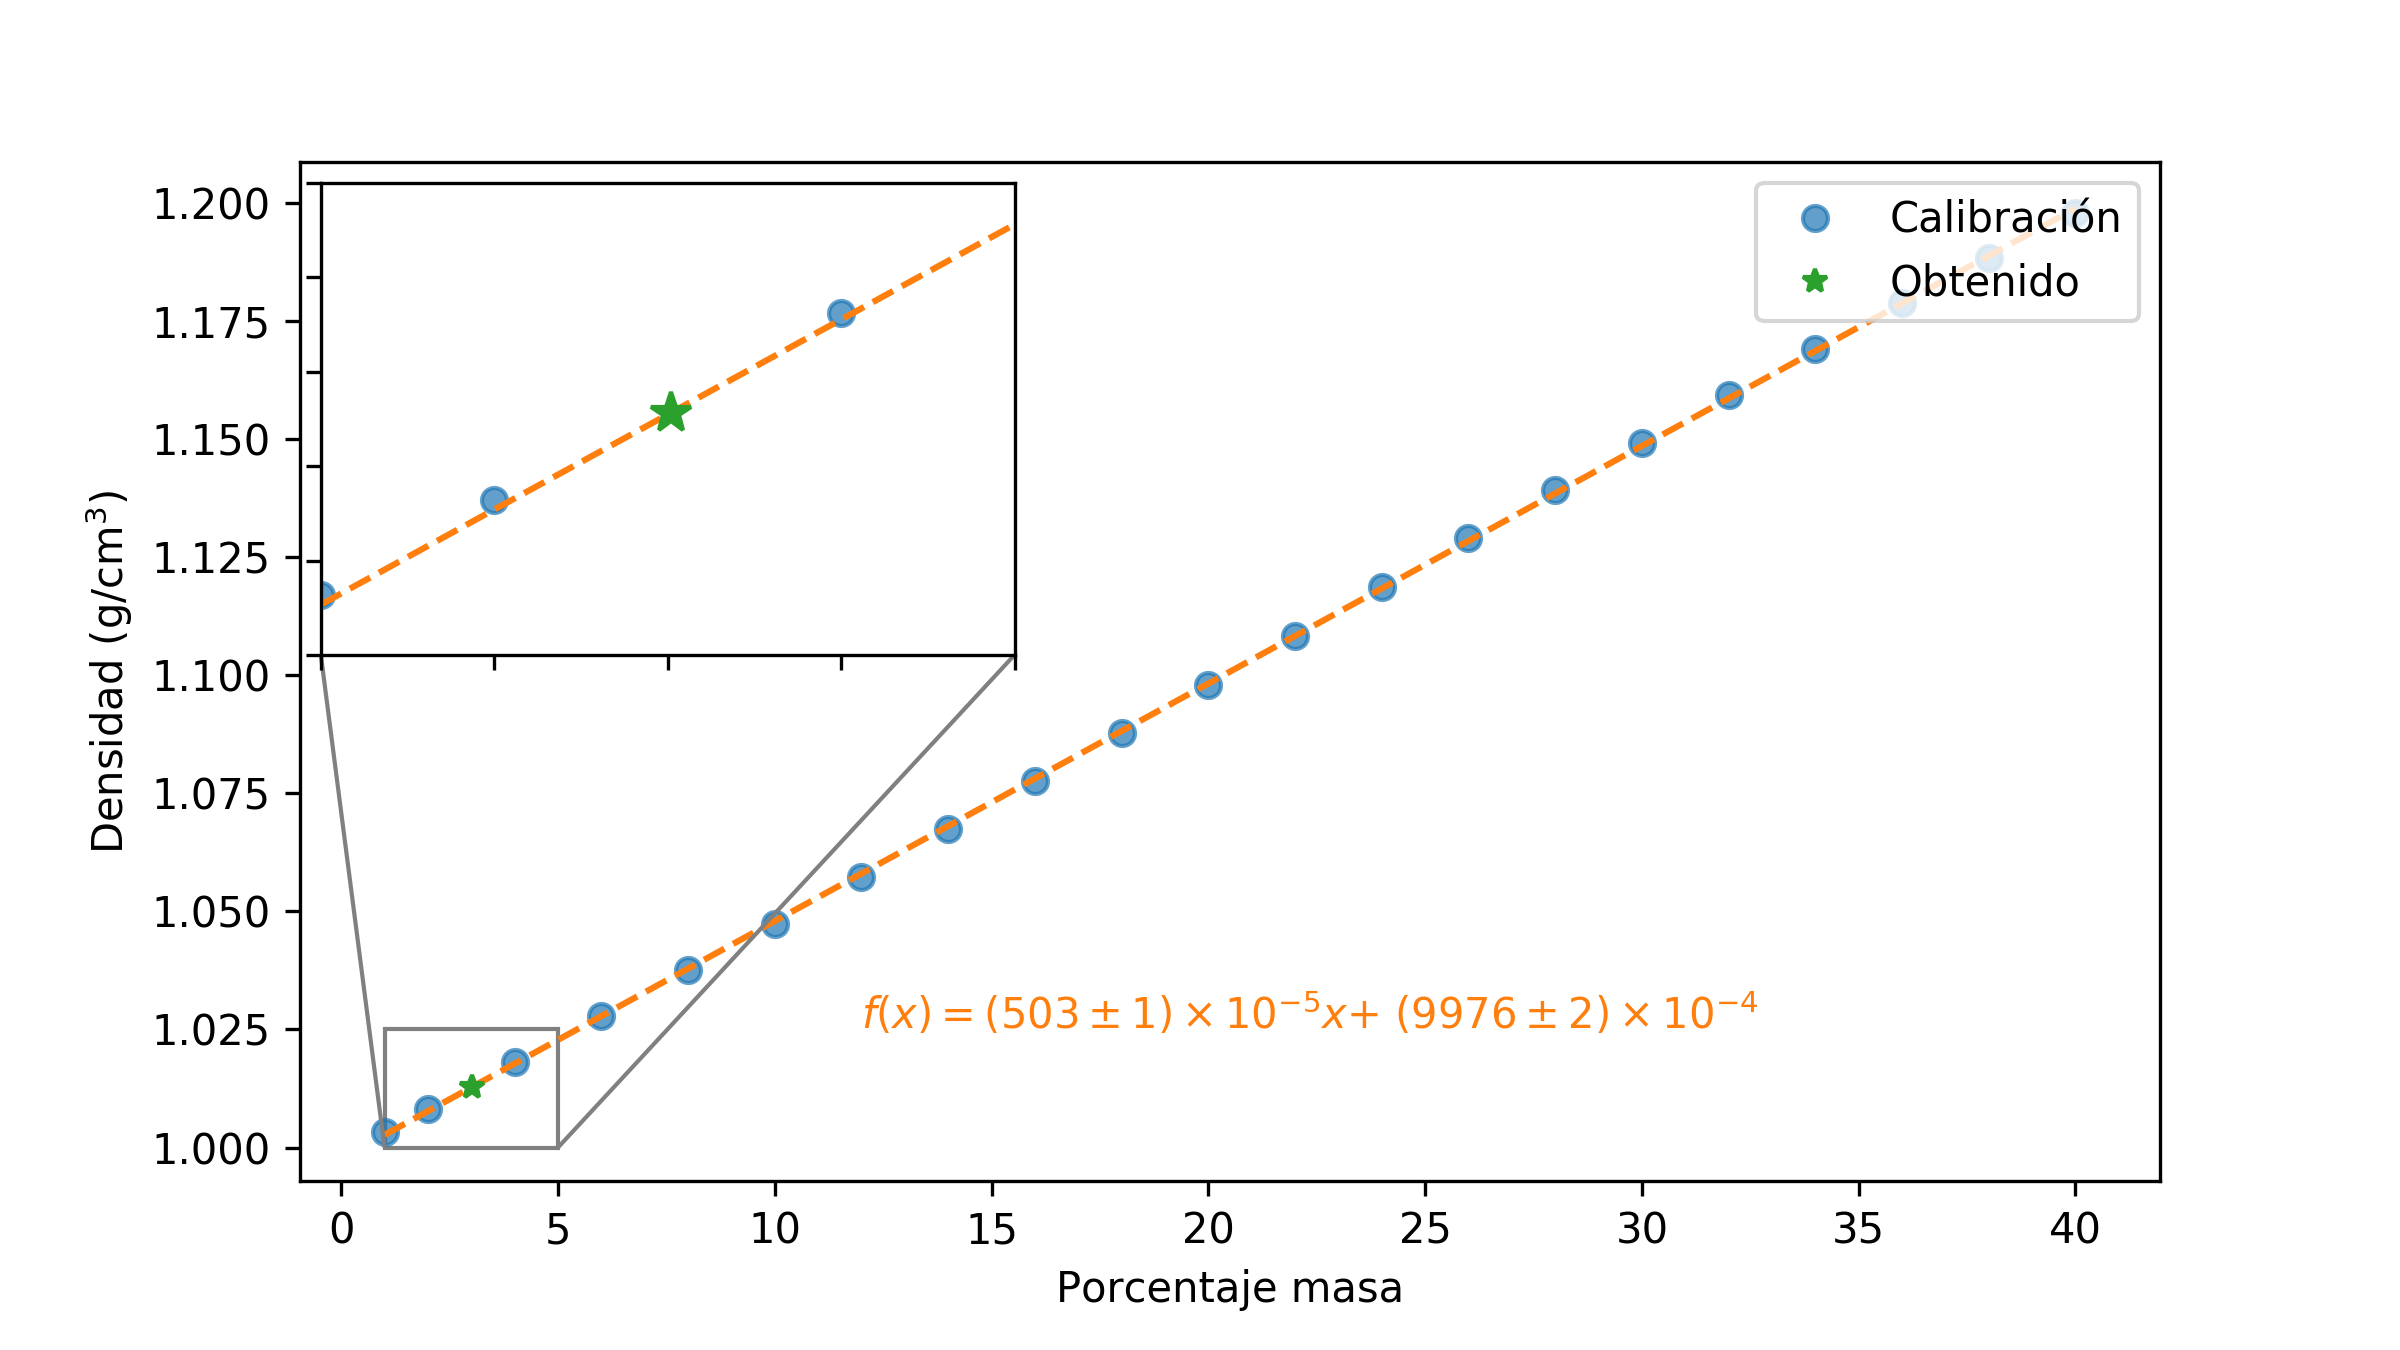
\includegraphics[width=\linewidth]{../Data/Concentration/C_HCl_initial.png}
			\caption{Determinaci\'on de la concentraci\'on de una soluci\'on de HCl usando valores de densidad reportados en la literatura \cite{perry2007perry}.}
			\label{fig: HCl_density}
		\end{figure}
		
		Para obtener la concentraci\'on $0.84 \pm 0.04$ M, se usa la siguiente ecuaci\'on, la cual relaciona la concentraci\'on en fracci\'on de masa con la molaridad $[M]$:
		\begin{equation}
			[M] = 10\dfrac{[w_t]\rho}{m_m} \qquad \text{$m_m$ la masa molecular del HCl}
		\end{equation}
		
		Se tiene entonces que la incertidumbre en la concentraci\'on estar\'a dada por:
		\begin{equation}
			\delta [M] = [M]\sqrt{\delta[w_t]^2 + \delta\rho^2} 
		\end{equation}
		
		Una al\'icuota de 0.0297 g de esta soluci\'on fue disuelta en 99.5553 g de agua, dando lugar a una soluci\'on 0.2469 mM. Donde la concentraci\'on final se calcula a partir de las densidades de las soluciones inicial ($\rho_s$) y final ($\rho_f$), las masas de agua ($m_\text{\ce{H2O}}$) y de soluci\'on inicial ($m_s$) usando la siguiente ecuaci\'on:
		\begin{equation}
			[M]_f = [M]_i\dfrac{V_s}{V_f} = [M_i]\dfrac{m_s/\rho_s}{(m_s + m_{\text{\ce{H2O}}})/\rho_f} =  [M]_i\left(\dfrac{m_s}{m_s + m_{\text{\ce{H2O}}}}\right)\left(\dfrac{\rho_s}{\rho_f}\right)
		\end{equation}
		
		\begin{table}[h]
			\centering
			\begin{tabular}{c|cccccc}
				& $\mathbf{[M]_i}$ (M) & $\mathbf{m_s}$ (g) & $\mathbf{m_{\text{H2O}}}$ (g) & $\mathbf{\rho_s}$ (g/cm$^3$)& $\mathbf{\rho_f}$ (g/cm$^3$) & $\mathbf{[M]_f}$ (mM) \\
				\hline
				\textbf{\ce{HCl}} & $0.84 \pm 0.04$ & $0.0297$ & $99.5553$ & $1.012832$ & $0.998205$ & $0.24690$ \\
				\textbf{\ce{KHCO3}} & $0.1022577$ & $0.1709$ & $99.5657$ & $1.003662$ & $0.998215$ & $0.1742689$ \\
				\hline
			\end{tabular}
			\caption{Densidades y masas medidas para alcanzar las soluciones con concentraciones 0,25 mM y 0,17 mM para el HCl y \ce{KHCO3}.}
		\end{table}
		
	\subsection{Soluci\'on de \ce{KHCO3} 0.17 mM}
	En un bal\'on aforado de 10 mL fueron adicionados 0.10143 g de \ce{KHCO3}, junto con 9.93551 g de \ce{H2O}. La densidad fue medida a 25 $^\circ$C y su valor fue 1.003662 g/cm$^3$. La concentraci\'on de esta soluci\'on se calcul\'o usando la siguiente ecuaci\'on:
	\begin{equation}
		[M] = \dfrac{n}{V} = \dfrac{m\rho}{m_m(m + m_{\ce{H2O}})}
	\end{equation}

	Obteniendo un valor de $0.10100\pm 0.00001$ M, donde la incertidumbre se calcula usando:
	\begin{equation}
		\delta[M] = \sqrt{\frac{\delta\rho^{2} m^{2}}{m_m^{2} \left(m + m_{\text{\ce{H2O}}}\right)^{2}} + \frac{\delta m^{2} \rho^{2} m_{\text{\ce{H2O}}}^{2}}{m_m^{2} \left(m + m_{\text{\ce{H2O}}}\right)^{4}} + \frac{\delta{m_{\text{\ce{H2O}}}}^{2} \rho^{2} m^{2}}{m_m^{2} \left(m + m_{\text{\ce{H2O}}}\right)^{4}}}
	\end{equation}
\section{Sistema de inyecci\'on}
	\subsection{Calibraci\'on de la jeringa}
	\subsection{Control por software}
	
\section{Realizaci\'on del experimento}

\section{Resultados}


		